\documentclass[a4paper,11pt]{article}

% Packages
\usepackage{graphicx}   % for including figures
\usepackage{grffile}    % for graphicspath
\graphicspath{{figures/}} % set path for figures
\usepackage{caption}    % better captions
\usepackage{subcaption} % side-by-side figures with captions
\usepackage{float}      % for [H] placement
\usepackage{amsmath}    % for math symbols
\usepackage{geometry}   % page layout

\usepackage[hidelinks]{hyperref}
\geometry{margin=2cm}

\title{Cavity Analysis}
\author{Stefan Rau \\ Institute for Quantum Matter}
\date{\today}

\begin{document}

\maketitle
\tableofcontents
\newpage
\begin{center}
    \vspace{5cm}
    This document presents the analysis of the cavity with the photodiode (APD130A/M).
\end{center}
\newpage
\section{Large Scan}
Note: The analysis of this scan was later assumed to be incorrect, as it was found that the finesse is actually much higher. See more in section 5.
\subsubsection*{Settings}
Used settings:  \\
$f = 6.0$ Hz,  \\
Amplitude: 4.4 V,  \\
Offset: 370 mV.  \\
Filename: \texttt{ALL0002.CSV}.  


With these settings, the cavity presumably scanned over two FSRs.

\subsection{Full Trace}
Figure~\ref{fig:full} shows the full photodiode voltage (left axis) and the
sync voltage (right axis) as a function of time. The highlighted region
indicates the section of the data that was selected for further analysis (For comparison between sync voltage and piezo voltage, see Fig. \ref{fig:osci}).

\begin{figure}[H]
    \centering
    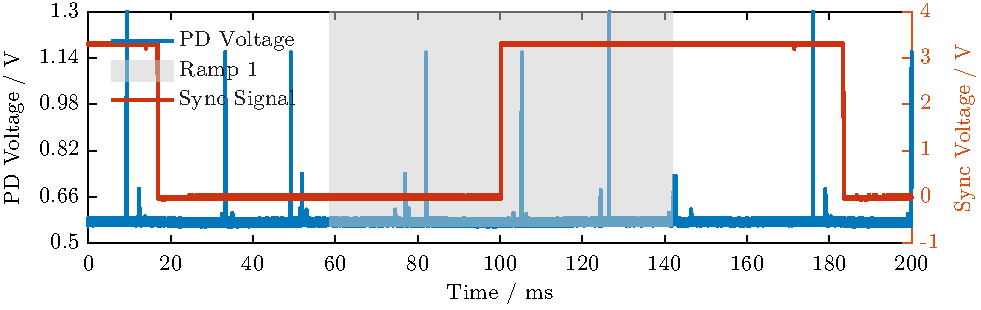
\includegraphics[width=\textwidth]{Figure_1.pdf}
    \caption{The rectangular signal is the sync signal of the function generator. The shaded region marks one ramp of the piezo (either increasing or decreasing the cavity length).}
    \label{fig:full}
\end{figure}

\subsection{Considered Region}
Figure~\ref{fig:fit} shows the selected region of the PD signal, normalized and
plotted with an Airy function. (This corresponds to Ramp 1 from the full trace.)

\begin{figure}[H]
    \centering
    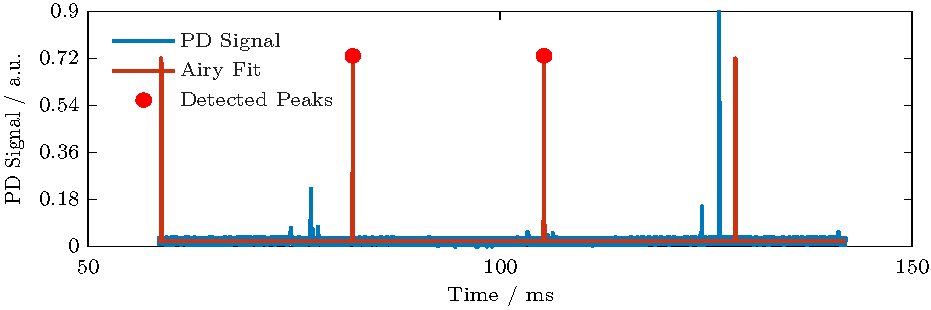
\includegraphics[width=\textwidth]{Figure_2.pdf}
    \caption{The two detected peaks lie directly underneath the fitted Airy function. The right-most peak is not well fitted, most likely due to non-linearity of the piezo scan.}
    \label{fig:fit}
\end{figure}

\subsection{Individual Peaks}
Each detected peak is shown separately in Figures~\ref{fig:peak1} and \ref{fig:peak2}.
Note that the span of the $x$-axis is chosen to be $10 \times$ FWHM of the fitted Airy.
The plotted finesse is $\mathcal{F}=2000$. This was done by guesstimating the finesse to get a good match.
A fit did not reliably work, which is why it was done manually.

\begin{figure}[H]
    \centering
    \begin{subfigure}[t]{0.48\textwidth}
        \centering
        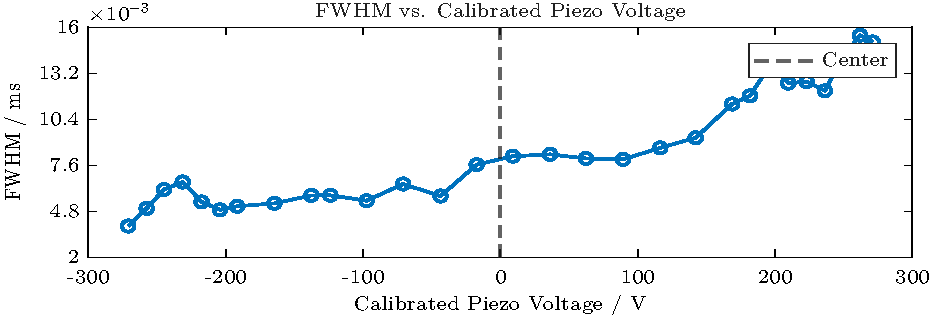
\includegraphics[width=\textwidth]{Figure_3.pdf}
        \caption{Zoomed-in view of Peak 1.}
        \label{fig:peak1}
    \end{subfigure}
    \hfill
    \begin{subfigure}[t]{0.48\textwidth}
        \centering
        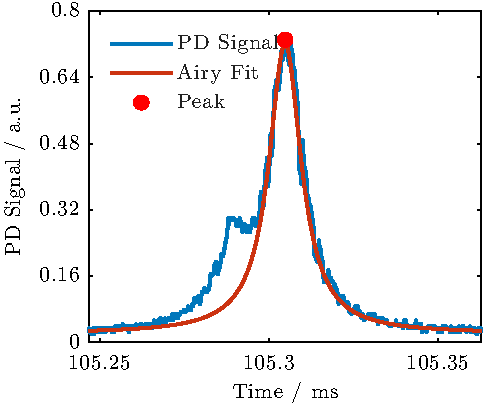
\includegraphics[width=\textwidth]{Figure_4.pdf}
        \caption{Zoomed-in view of Peak 2.}
        \label{fig:peak2}
    \end{subfigure}
    \caption{Zoomed-in views of the detected peaks in the selected region.}
\end{figure}

\newpage
\section{Lower Voltage}
\subsubsection*{Settings}
Used settings:  \\
$f = 6.0$ Hz,  \\
Amplitude: 2.3 V,  \\
Offset: -120 mV.  \\
Filename: \texttt{ALL0003.CSV}.  

\subsection{Full Trace}

\begin{figure}[H]
    \centering
    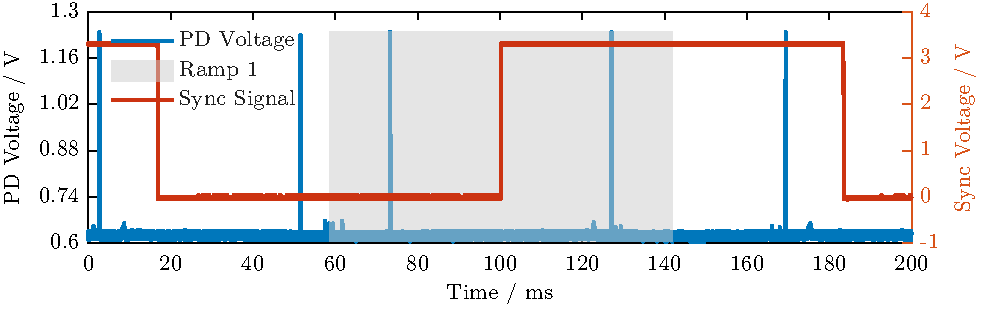
\includegraphics[width=\textwidth]{Figure_1_low.pdf}
    \caption{The rectangular signal is the sync signal of the function generator. The shaded region marks one ramp of the piezo (either increasing or decreasing the cavity length).}
    \label{fig:full_low}
\end{figure}

\subsection{Considered Region}
same as previous
\begin{figure}[H]
    \centering
    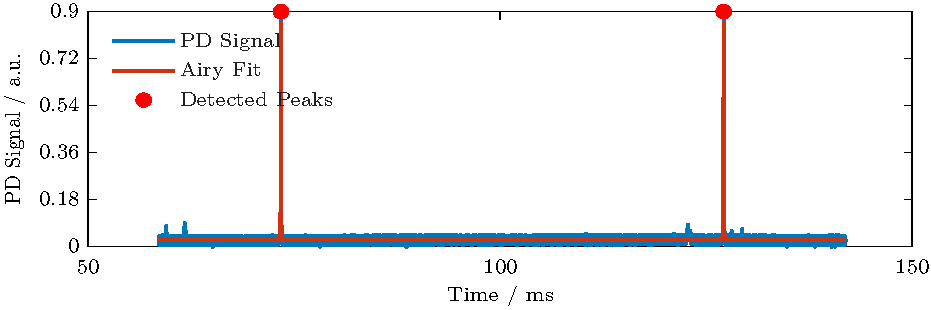
\includegraphics[width=0.9\textwidth]{Figure_2_low.pdf}
    \caption{The two detected peaks lie directly underneath the fitted Airy function. The right-most peak is not well fitted, most likely due to non-linearity of the piezo scan.}
    \label{fig:fit_low}
\end{figure}

\newpage
\subsection{Individual Peaks}
The plotted finesse is once again $\mathcal{F}=2000$.

\begin{figure}[H]
    \centering
    \begin{subfigure}[t]{0.48\textwidth}
        \centering
        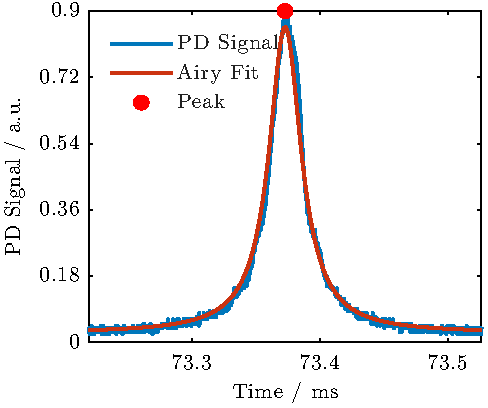
\includegraphics[width=\textwidth]{Figure_3_low.pdf}
        \caption{Zoomed-in view of Peak 1.}
        \label{fig:peak1_low}
    \end{subfigure}
    \hfill
    \begin{subfigure}[t]{0.48\textwidth}
        \centering
        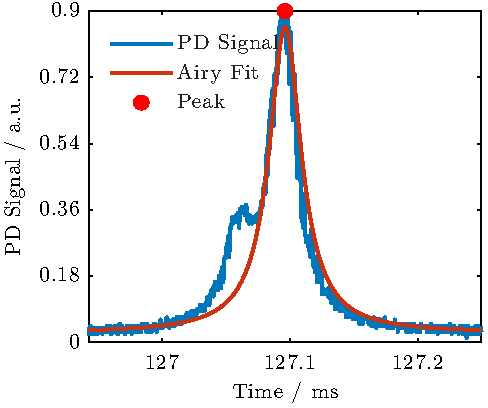
\includegraphics[width=\textwidth]{Figure_4_low.pdf}
        \caption{Zoomed-in view of Peak 2.}
        \label{fig:peak2_low}
    \end{subfigure}
    \caption{Zoomed-in views of the detected peaks in the lower-voltage scan.}
\end{figure}

\newpage
\section{Piezo Ramp Analysis (Piezo 2)}
\subsubsection*{Settings}

$f = 5.0$ Hz,  \\
Amplitude: 5.2 V,  \\
Offset: 0 V.  \\
Filename: \texttt{ALL0007.CSV}.   \\
Piezo No.; \texttt{2}  \\
Script: \texttt{overlayRamps.m} \\


In this, I try to understand the hystereis of the piezo. For this, I scanned several ramps and overlaid them.
I sorted them by High-Low and Low-High ramps. The results are shown in Figures~\ref{fig:fit_low} to \ref{fig:fit_low}.


\begin{figure}[H]
    \centering
    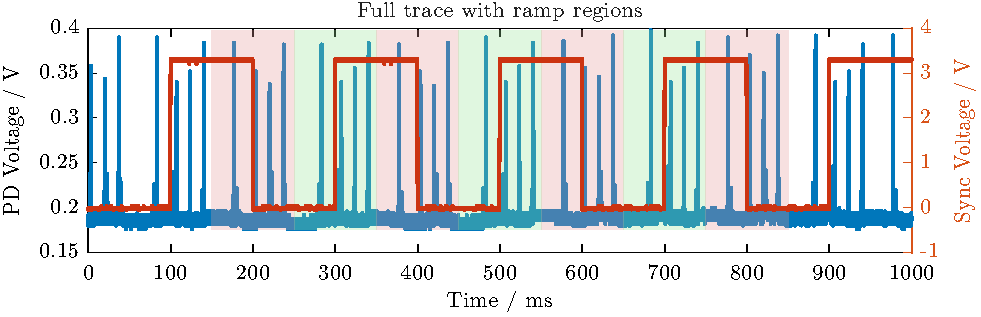
\includegraphics[width=\textwidth]{ManyRamp/ManyRamps.pdf}
    \caption{High-Low-Ramp: Red, Low-High-Ramp: Green}
\end{figure}

\begin{figure}[H]
    \centering
    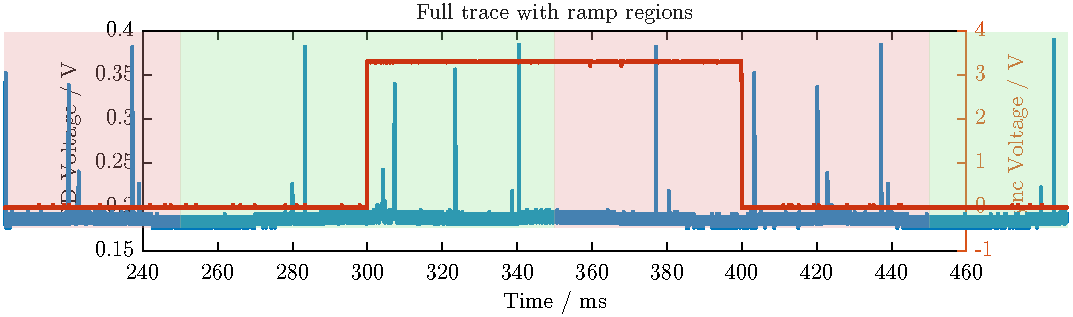
\includegraphics[width=\textwidth]{ManyRamp/Zoomed_Ramp.pdf}
    \caption{Zoom in section from the previous figure. It is worth mentioning that the peaks are not symmetrically spread around the turning point for the piezo. The turning point is at the border between a red and a green area.}
\end{figure}

\newpage

\begin{figure}[H]
    \centering
    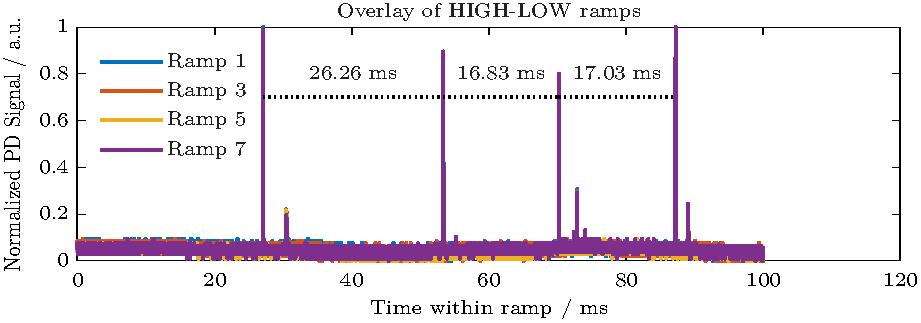
\includegraphics[width=\textwidth]{ManyRamp/HiLo.pdf}
    \caption{Here, I overlaid all the High-Low ramps and determined the average peak distance. It seems that it is not linear.}
\end{figure}

\begin{figure}[H]
    \centering
    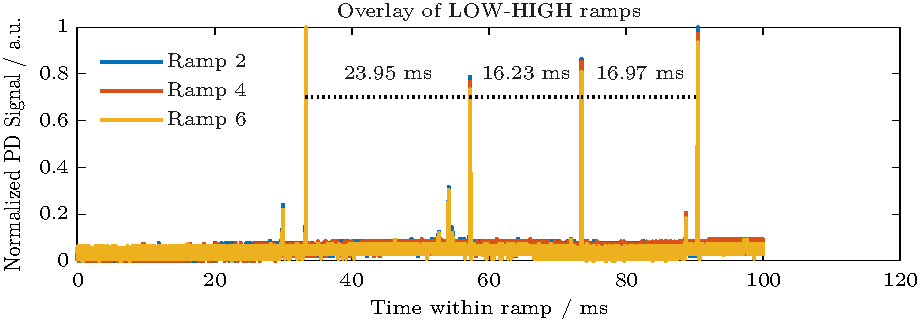
\includegraphics[width=\textwidth]{ManyRamp/LoHi.pdf}
    \caption{Same with this figure, but for the Low-High ramps.}
\end{figure}

It is super strange to me that the peak distances seem so arbitrary. 
You need to keep in mind that the piezo was moving in the \textbf{opposite} direction for each of the above figures, however, the distances do not seem to be mirror images of each other.
I would have expected that the distances are the same, just mirrored. But they are not.
When looking at the smaller surrounding peaks, it is obvious that the piezo changed direction (in the first figure, the smaller peaks are behind the large peak - in the second figure they are in front of them).
I do not have a good answer for this behavior. Perhaps, the FSR is not between these two similarly sized peaks, but between two different ones.
If this were true, the finesse may perhaps be up to three times higher.
\newpage
\subsection{Other Piezo (Piezo 1)}
The switch to the second piezo did not change the signal noticeably.
Same settings as before, just a different piezo. File used \texttt{ALL0008.CSV}, Piezo No. \texttt{1}.
\begin{figure}[H]
    \centering
    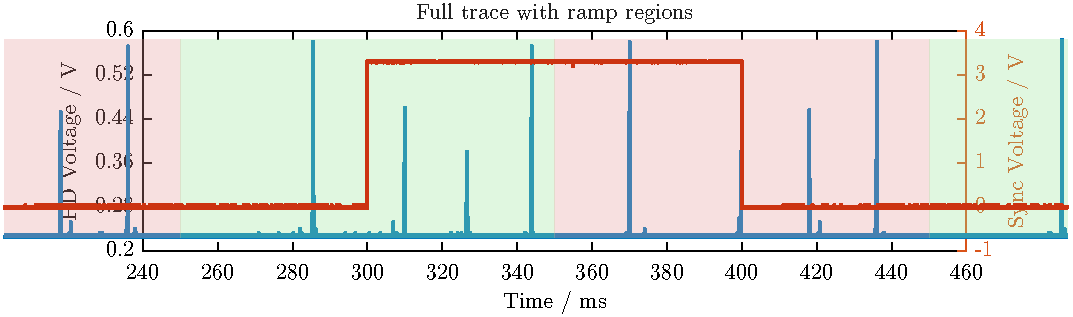
\includegraphics[width=\textwidth]{ManyRamp/Zoomed_Ramp2.pdf}
    \caption{Same as before, but with a different piezo.}
\end{figure}


\begin{figure}[H]
    \centering
    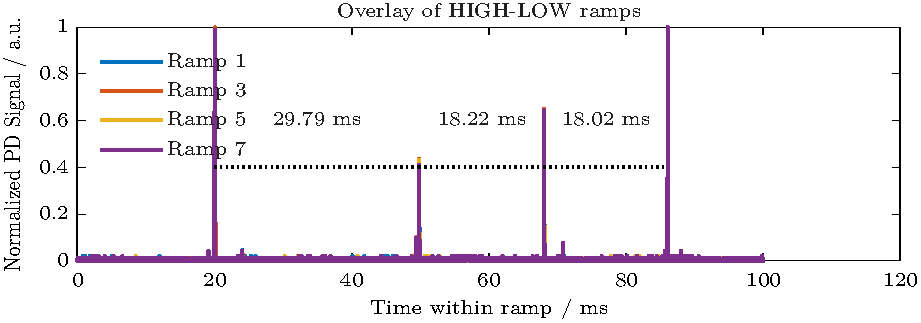
\includegraphics[width=\textwidth]{ManyRamp/HiLo2.pdf}
    \caption{Same as before, but with a different piezo.}
\end{figure}

\begin{figure}[H]
    \centering
    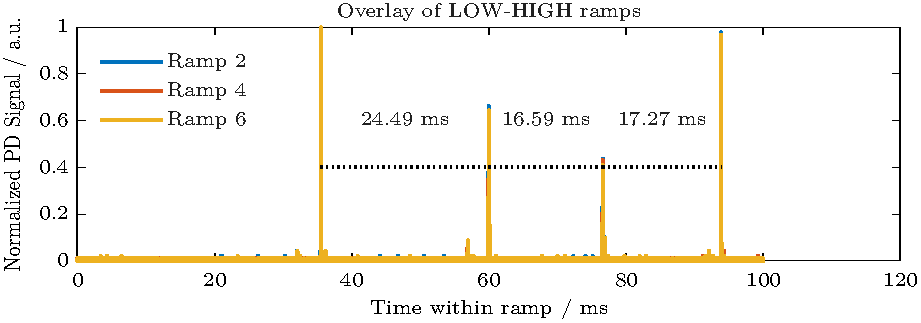
\includegraphics[width=\textwidth]{ManyRamp/LoHi2.pdf}
    \caption{Same as before, but with a different piezo.}
\end{figure}

\newpage
\section{Dual-Piezo Setup}
\subsubsection*{Scan-Settings}
$f = 6.0$ Hz,  \\
Amplitude: 5.2 V,  \\
Offset: 0 V.  \\
Filename: \texttt{ALL0010.CSV}.   \\
Piezo No.; \texttt{2}  \\
Script: \texttt{plotPdPiezo.m} \\

I now tried to use both piezos simultaneously. One piezo was used to scan the cavity length, the other was used to moved the peaks relative to the cavity scan.
To do this, a DC voltage was applied to the second piezo. This lead to a constant offset between the two mirrors, thus moving the peaks around whilst not interfering with the cavity scan.

This also allowed us to get a better feeling for the behaviour of the cavity. 
We therefore assume, that the prior analysis of a 2000 finesse is \textbf{incorrect}.
We coupled light to the cavity such that there are now two prominent peaks.
Startin off with no offset, we get the following:


\begin{figure}[H]
    \centering
    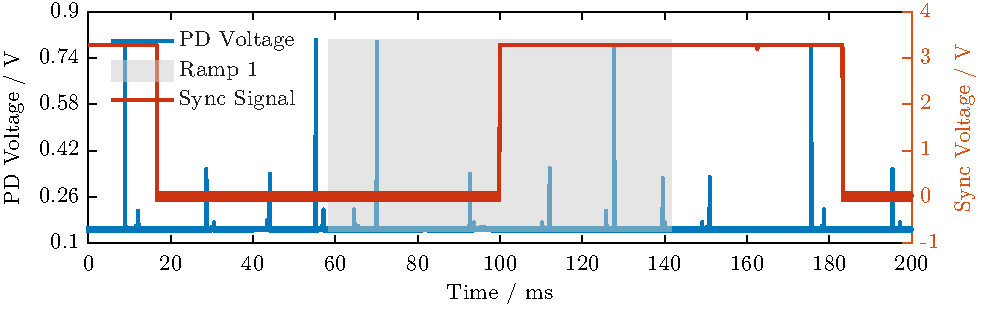
\includegraphics[width=\textwidth]{twoPiezo/Figure_1.pdf}
    \caption{The offset in this case was 0V.}
\end{figure}



\begin{figure}[H]
    \centering
    \begin{subfigure}[t]{0.48\textwidth}
        \centering
        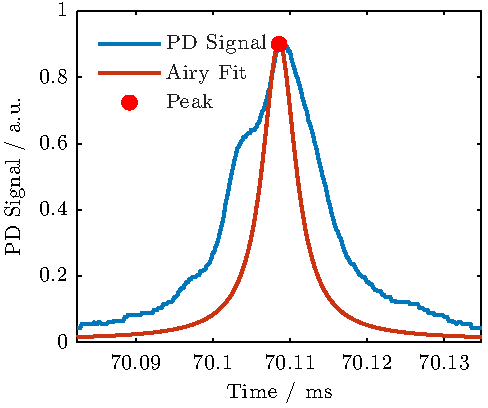
\includegraphics[width=\textwidth]{twoPiezo/Figure_3.pdf}
        \caption{Zoomed-in view of Peak 1.}
        \label{fig:peak1_0v}
    \end{subfigure}
    \hfill
    \begin{subfigure}[t]{0.48\textwidth}
        \centering
        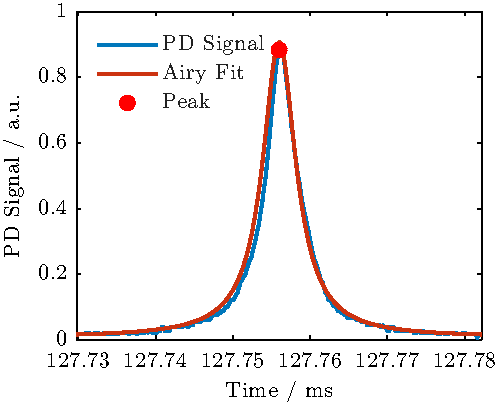
\includegraphics[width=\textwidth]{twoPiezo/Figure_4.pdf}
        \caption{Zoomed-in view of Peak 2.}
        \label{fig:peak2_0v}
    \end{subfigure}
    \caption{Zoomed-in views of the detected large peaks of one scan. The left one is cleary fuzzy and spread out.}
\end{figure}
This data corresponds to a finesse of $\mathcal{F}\approx11\,000$ - \textbf{much higher} than the previous value!
\newpage
\subsection{Offset 306V - Different FSR}
I tried to offset the peaks using the piezo (at 306 V) to see to different peaks in order to increase the quality of the left peak. 
However, this did not work.
When moving the right peak (here: peak 2 in Fig. \ref{fig:peak2_0v}) to the left of the frame (where currently peak 1 (Fig. \ref{fig:peak1_0v}) sits), it then gets fuzzy. 
So this means that the peak itself is not the issue, but perhaps the scan is not reliable in this region. This will later be analyzed.

It was however possible to see a new peak coming in from the right.
This is a good sign! 
This peak was of a good "qualitiy". In genereal, changing the offset of the second piezo did \textbf{not} change the signal much, but it made it possible to move the peaks around.


\begin{figure}[H]
    \centering
    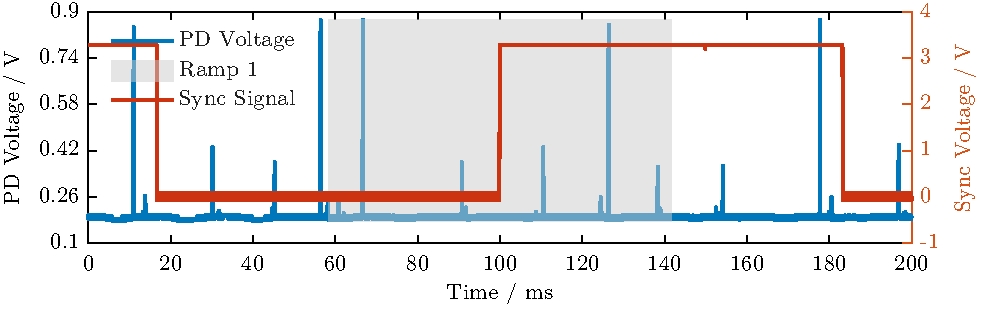
\includegraphics[width=\textwidth]{twoPiezo/Figure_11.pdf}
    \caption{Using the second piezo to move around the peaks, it was possible to see a new peak of similar and large amplitude. The offset in this case was 306V. File used: \texttt{ALL0015.CSV}}
\end{figure}


\begin{figure}[H]
    \centering
    \begin{subfigure}[t]{0.48\textwidth}
        \centering
        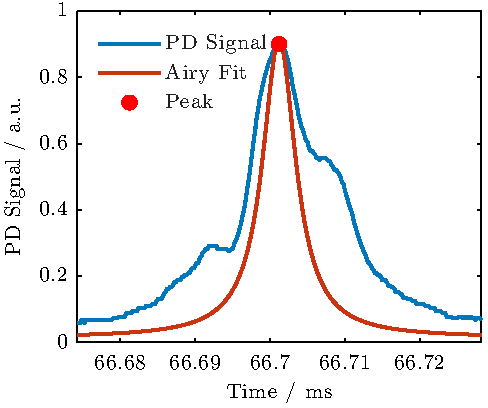
\includegraphics[width=\textwidth]{twoPiezo/Figure_31.pdf}
        \caption{Zoomed-in view of Peak 1.}
        \label{fig:peak1_low}
    \end{subfigure}
    \hfill
    \begin{subfigure}[t]{0.48\textwidth}
        \centering
        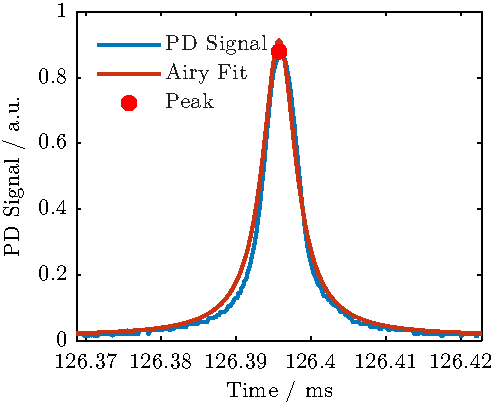
\includegraphics[width=\textwidth]{twoPiezo/Figure_41.pdf}
        \caption{Zoomed-in view of Peak 2.}
        \label{fig:peak2_low}
    \end{subfigure}
    \caption{Zoomed-in views of the detected large peaks of one scan. The left one is cleary still fuzzy and spread out.}
\end{figure}

Once again, this data corresponds to a finesse of $\mathcal{F}\approx11\,000$.

\newpage
\section{FWHM change on piezo position}
Using the dual-piezo setup, we decided to analyze the hysteresis of the piezo. To do this, the scan was once again actiaveted with the following setting:
\subsubsection*{Scan-Settings}
$f = 6.0$ Hz,  \\
Amplitude: 5.2 V,  \\
Offset: 0 V.  \\
Piezo No.; \texttt{2}  \\
Script: \texttt{analyzeFWHMvsPiezo.m} \\

The second piezo was used to change the position of the peaks using a DC offset voltage.
I changed to position of an arbitrary large Peak from the left most side of the scan to the right most side of the scan. I recorded the transmission signal for dozens of piezo offset voltages in order to see a change. Ideally, the relative position of the peak compared to the scan should not matter, but as seen previously, it does. 


\begin{figure}[H]
    \centering
    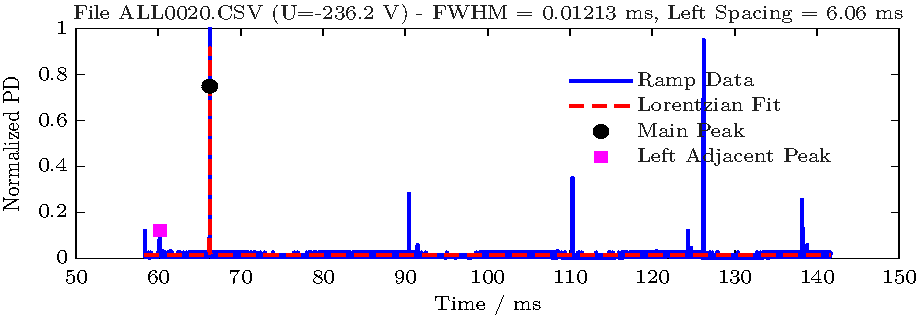
\includegraphics[width=\textwidth]{fwhm/Figure_1.pdf}
    \caption{Example frame, where the peak investigated is still fairly to the left of the scan. The x axis has been cut-off to represent only the length of one direction of a scan (here roughly from 58 to 143 ms). The position of main peak is marked in black (this does not indicate the fitting, only the position on the x axis) and a second peak has been marked in pink, which will also be used for analysis.}
\end{figure}


\begin{figure}[H]
    \centering
    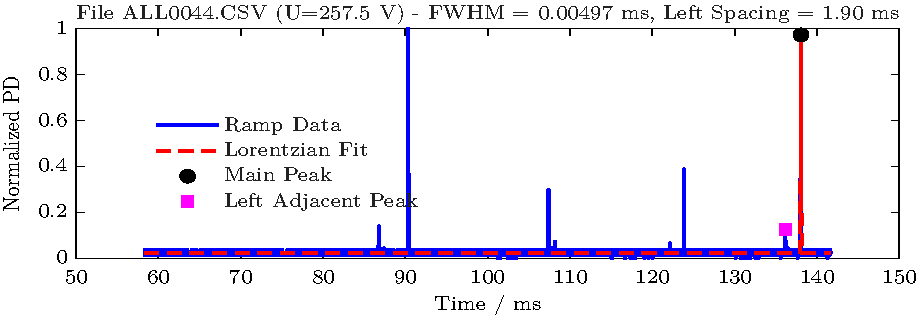
\includegraphics[width=\textwidth]{fwhm/Figure_2.pdf}
    \caption{Now, the two peaks have moved to the right side of the scan. Clearly, the time distance between the peaks has gotten shorter. Also, if you look at the title, the FWHM has also shrunk.}
\end{figure}

The FWHM have been determined by a Lorentzian Fit around the peak. I made sure to always analyze the same peak. Combining dozens of offset voltages, we get the following plots showing the FWHM deviation as well as the spacing between the two adjacend peaks. The x axes have been scaled to show the voltage of the scanned piezo at the position of the peak


\begin{figure}[H]
    \centering
    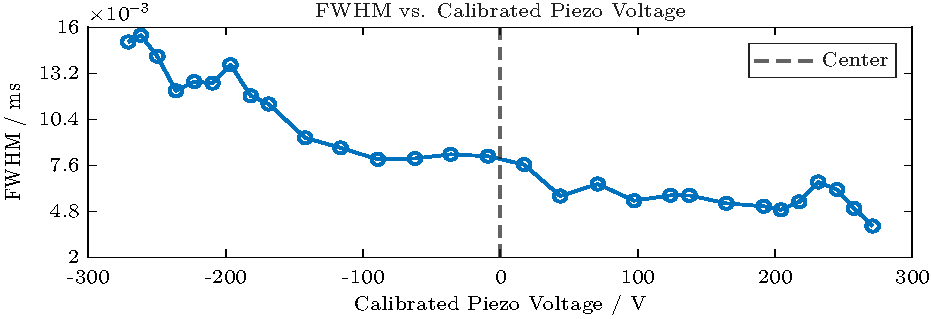
\includegraphics[width=\textwidth]{fwhm/Figure_3.pdf}
    \caption{This plot shows the change in FWHM coming from one side of the scan the other. It is clear that the FWHM did change significantly (by a factor of around 3.8). The x axis represents the voltage of the scanning piezo for each peak position.}
\end{figure}


\begin{figure}[H]
    \centering
    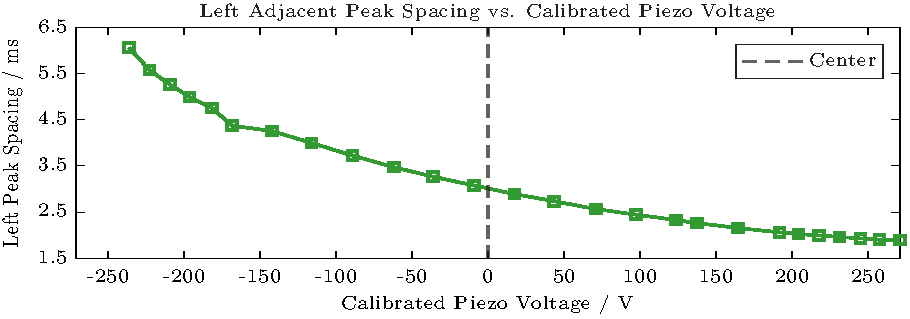
\includegraphics[width=\textwidth]{fwhm/Figure_4.pdf}
    \caption{Once again, the distance between the two adjacend peaks differs significantly from one side to the other with a factor of 3.2 (this cant be directly compared to the previous factor, as the adjacent peak was not captured in the first couple of measurements. If we compare the range where both the FWHM and the peak distances has been captured, this factor is nearly identical)}
\end{figure}

Unfortuneatley, it seems that during the run of this measurements, the piezo that was used with a DC offset voltage has been damaged. 

\newpage
\section{Cavity with EOM sidebands}
Now, we switched lasers to a 767nm laser and also added an EOM to add sidebands to the laser.
The goal was to measure the linewidth of the cavity peaks more accurately, since we now know that the pizeo is highly unlinear.

In the following, two finesse values will be presented: 
\begin{itemize}
    \item Finesse (distance): This is the ratio between the distance of two adjacent cavity peaks and the FWHM of a peak. Both are measured in ms using the oscilloscpe data. This is similar to just fitting an Airy function
    \item Finesse (500 GHz): Here, the FWHM of a peak is measured using the EOM sideband calibration, thus allowing us to compensate for any piezo hysteresis. The distance is then assumed to be 500 GHz, which should be $\approx \pm 10\%$ of the actual value. This was calculated using $\Delta \nu = \frac{c}{2L}$ with $L\approx300 \mu m$.
\end{itemize}


\begin{figure}[H]
    \centering
    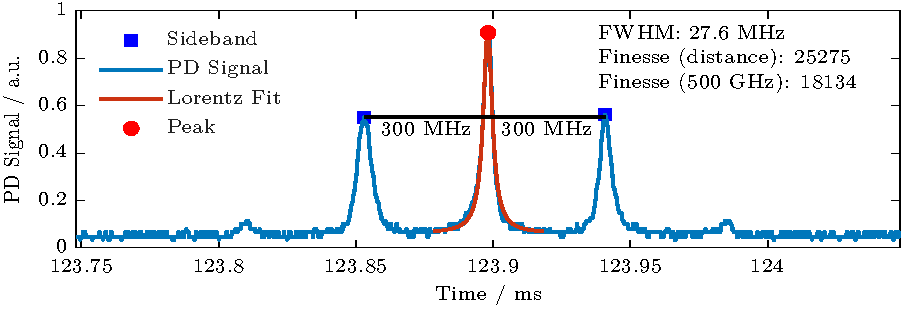
\includegraphics[width=\textwidth]{EOM/Peak2.pdf}
    \caption{Here, the EOM has created two noticable sidebands at a distance of 300 MHz. Knowing this, it was possible to calibrate the time domin to a frequency domain and thus determining the FWHM of the peak. Note that the Finesse is still only given using the non-calibrated time-domain, as we can\'t easily compensate for the non-linearity of the piezo. Also, for this figure, individual Lorentzian peaks have been fitted instead of an entire Airy function. This allowed us to get a kind-of lower and upper-case estimate for the finesse, using both FWHM values for each peak.}
\end{figure}

\begin{figure}[H]
    \centering
    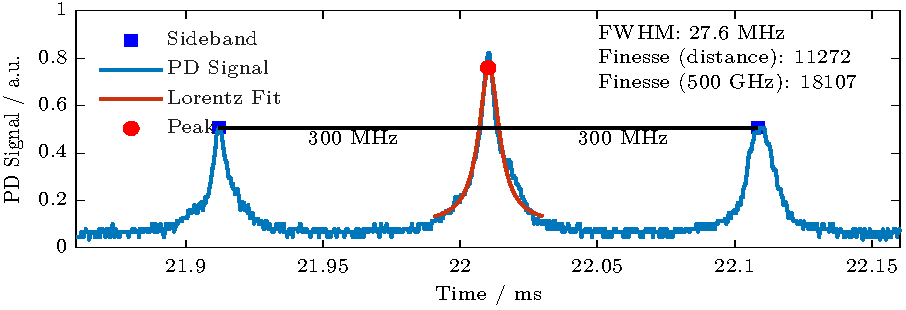
\includegraphics[width=\textwidth]{EOM/Peak1.pdf}
    \caption{Here, the second peak is shown. The x axis scale shows the same time length (0.4 ms) as in the previous figure.}
\end{figure}


Laser issues, worse results possible, calculate over 500 GHz is more reliable

A few things to mention: The laser was not super stable. The above plots are among the best ones that we\'ve been able to capture. For many laser configurations (temperature, power), we saw multimode bevahiour of the cavity.
In some measurements, the calibrated FWHM also differed by up to 30\% between each peak.

Additionally, the difference in the Finesse (distance) and the Finesse (500 GHz) once again shows the non-linear bevahiour of the piezo.
The left peak tends to undererstimate the finesse, whilst the right one tends to overerstimate it. The correct value most likely lies somewhere inbetween.

\newpage
\section{Looking at the backreflex}
We now placed the PD on the backreflecting light beam. So now, we expect to see dips instead of peaks in our signal.


\begin{figure}[htbp]
    \centering
    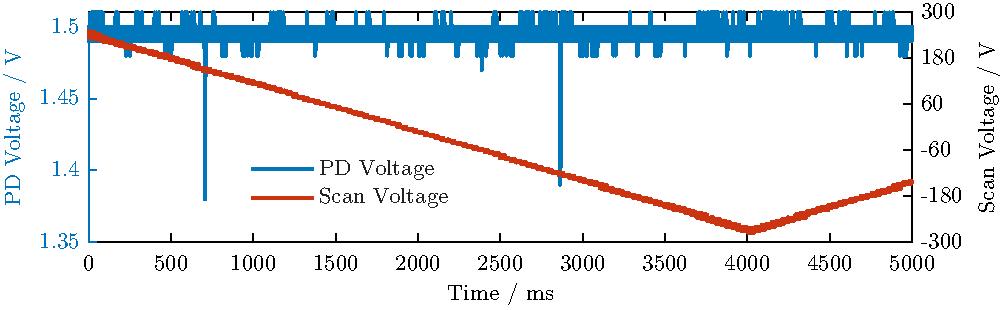
\includegraphics[width=\textwidth]{back/Figure_1.pdf}
    \caption{Here, we see dips instead of peaks. The red curve now accurately shows the piezo scan voltage. This was achievable by setting up a function generator with two synced outputs. By choosing the same settings for both outputs (12 Hz and 2.7 V peak tp peak) and then matching their phase, this signal should be an accurate representation of the piezo scan voltage.}
\end{figure}
Now, I inverted the signal in order to be able to use my existing code for further analysis. I kept the EOM running to compare the FHWM.

\begin{figure}[htbp]
    \centering
    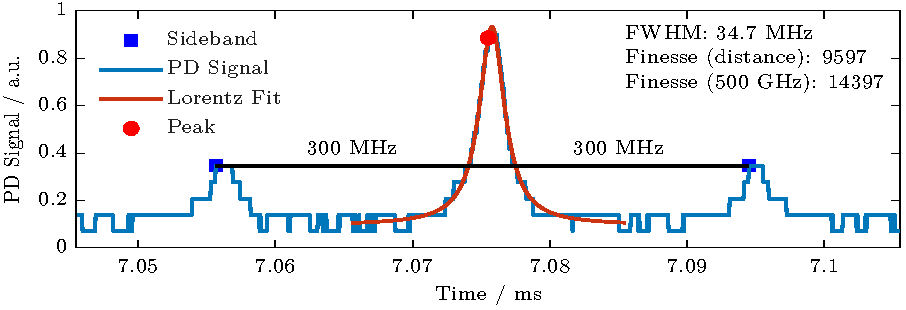
\includegraphics[width=\textwidth]{back/Figure_3.pdf}
    \caption{Zoomed in on one peak with its sidebands.}
\end{figure}
\begin{figure}[htbp]
    \centering
    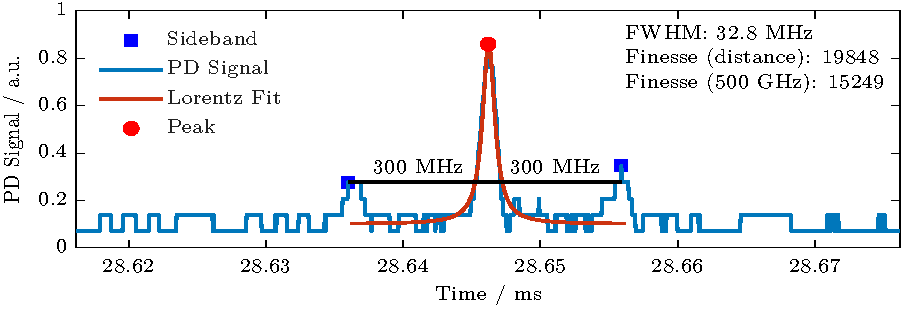
\includegraphics[width=\textwidth]{back/Figure_4.pdf}
    \caption{Zoomed in on antoher peak with its sidebands.}
\end{figure}

The FWHM values appear slightly larger than in the previous transmission setup.
However, due to the high noise level, the sideband peak detection is less accurate than before.
When the detector was placed back on the transmission side, the FWHM values matched in both cases (within 10\%). 
So perhaps the measurement in the previous section was just lucky.

The EOM was set to 10 dBm instead of the previous 12 dBm (at the transmission setup) to try to preserve the central cavity peak as much as possible. 
The EOM cuts away intensity from the central peak, which makes it harder to make out.
All in all, the backreflecting light shows similar finesse values than the transmission side. 

\newpage
\section{Setup}
\begin{figure}[htbp]
    \centering
    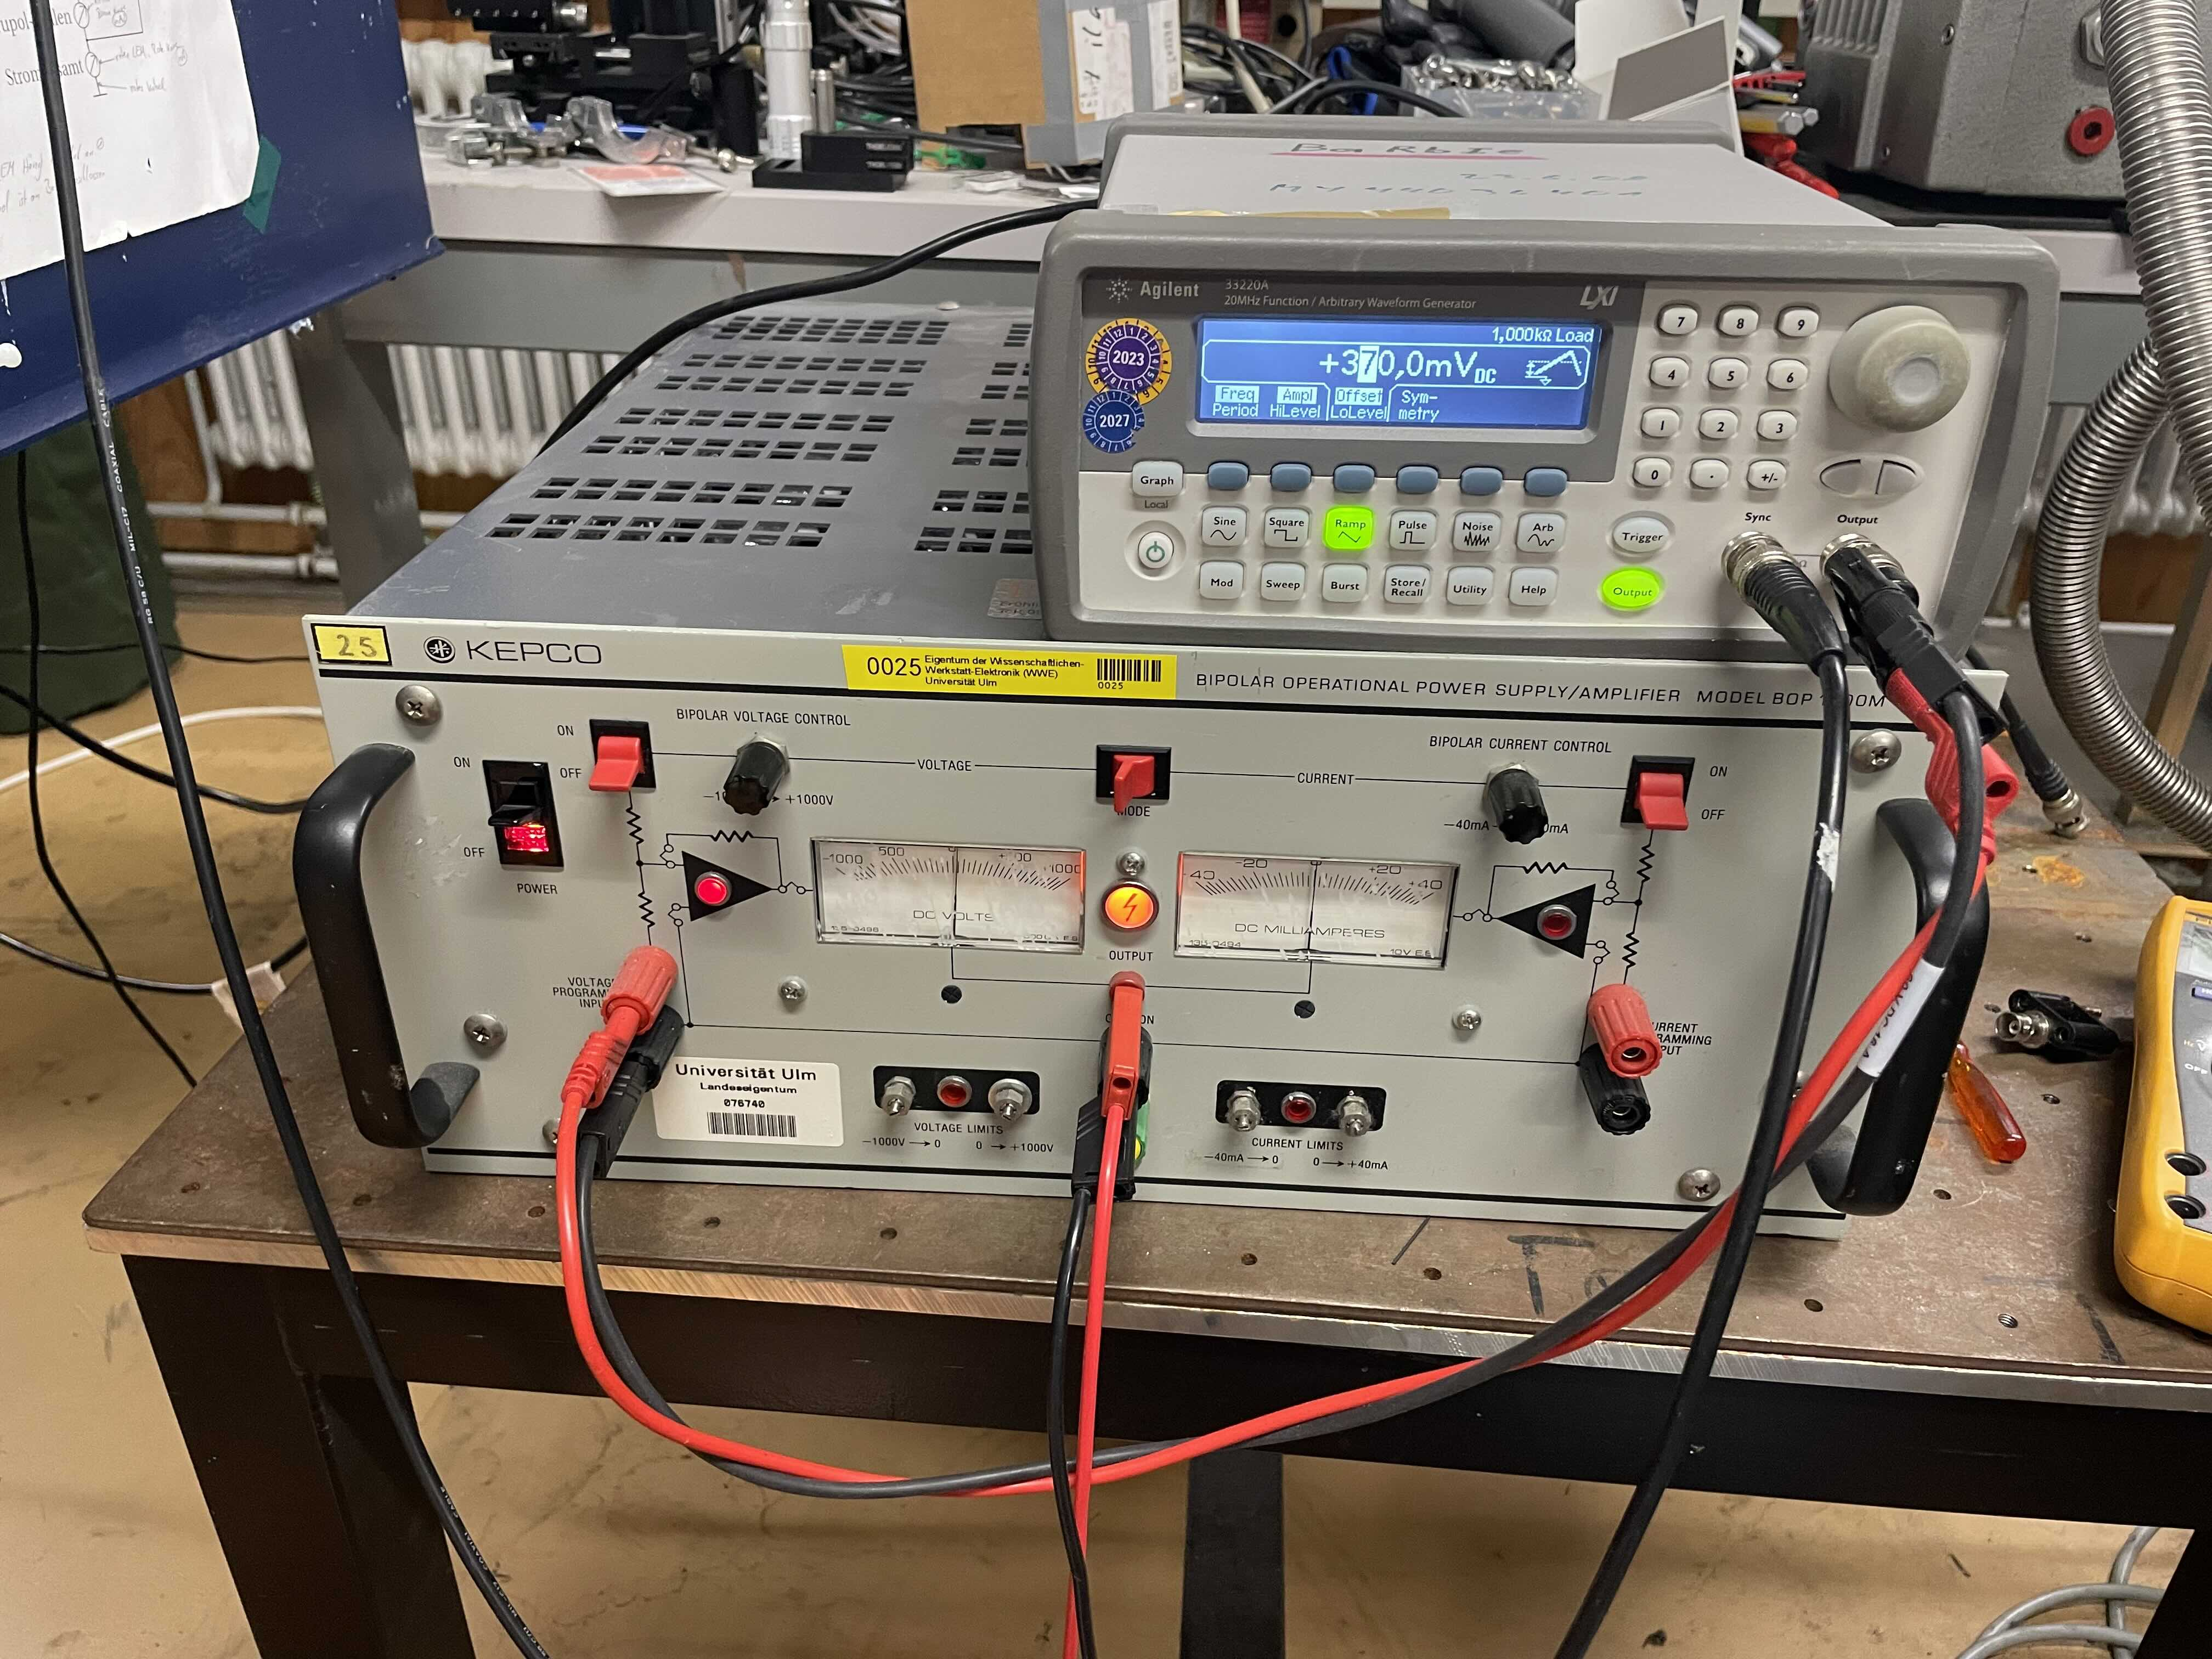
\includegraphics[width=\textwidth]{IMG_8997.jpg}
    \caption{HV Amplifier setup with function generator. Do \textbf{not} exceed the piezo voltage rating. It can only handle $\pm 320$~V at absolute max. We set the limiter light to around 250~V to avoid overshooting.}
\end{figure}

\begin{figure}[htbp]
    \centering
    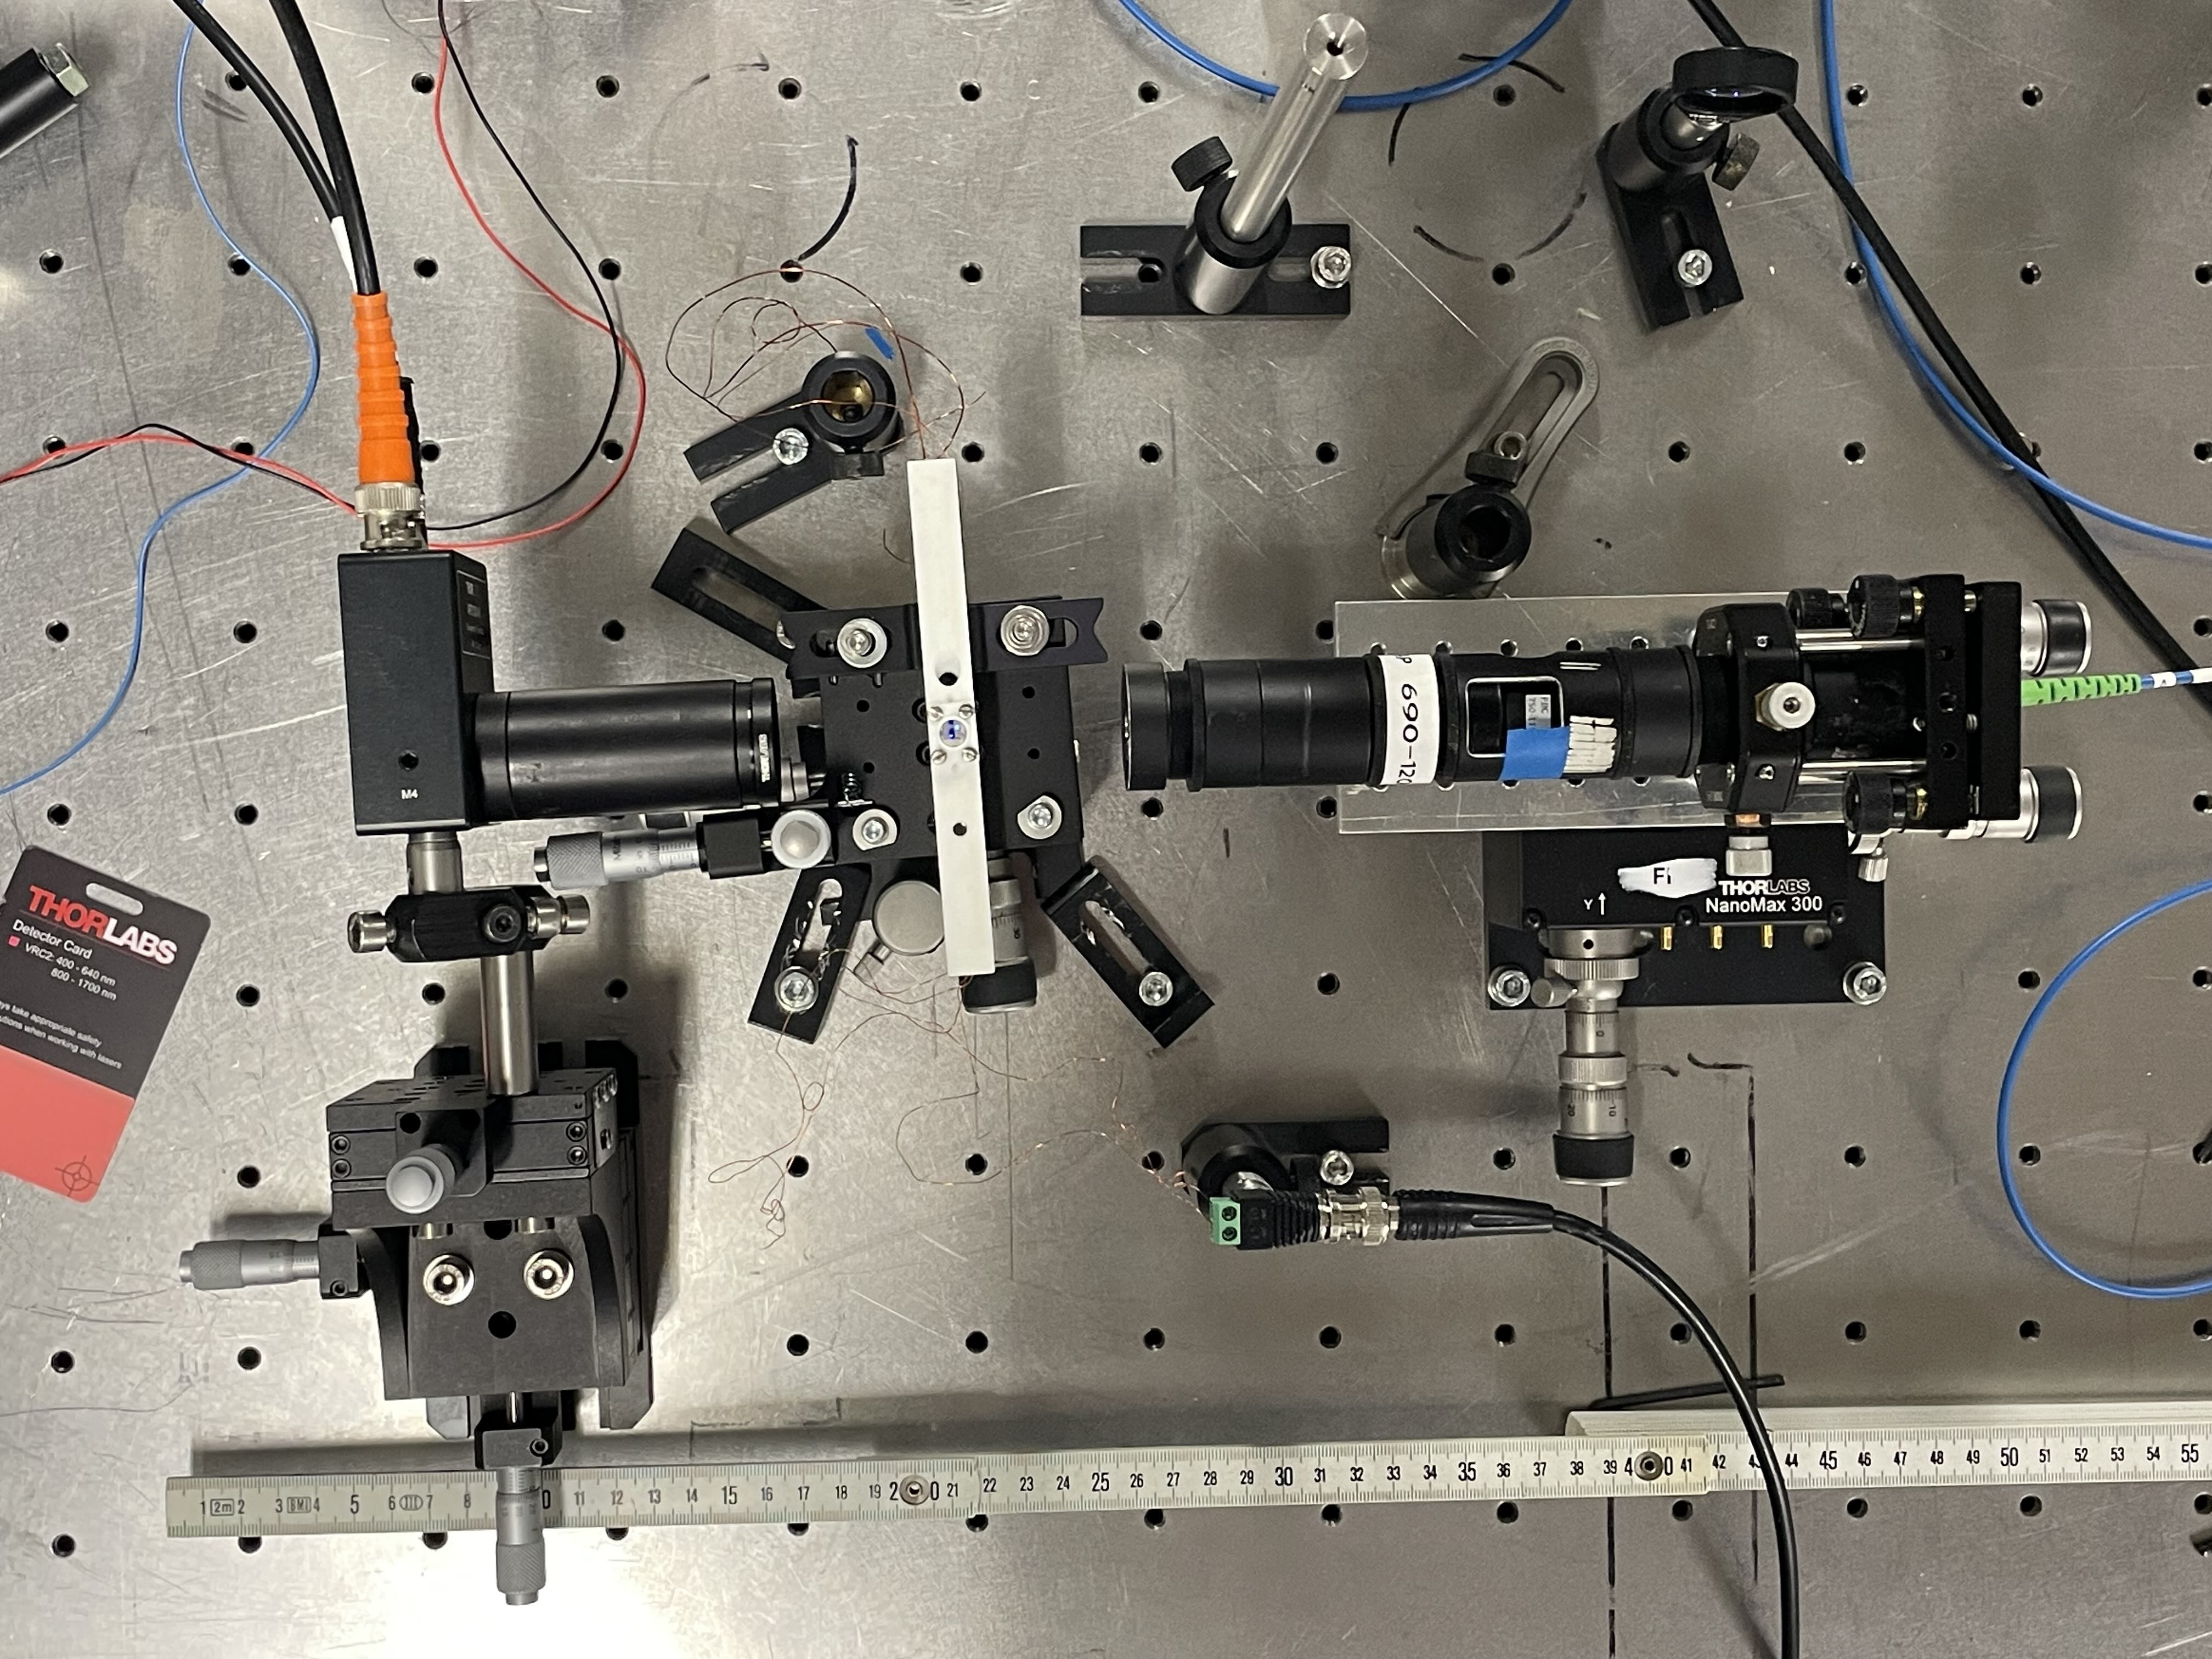
\includegraphics[width=\textwidth]{IMG_8999.jpg}
    \caption{Cavity setup from top view. PD is on the left, incident light is on the right. Incoupling light, cavity and PD are all mounted on individual $xyz$-translation stages. In front of the PD, there is a lens ($f=25.1$~mm) to focus the light onto the sensor.}
    \label{fig:setup}
\end{figure}

\begin{figure}[htbp]
    \centering
    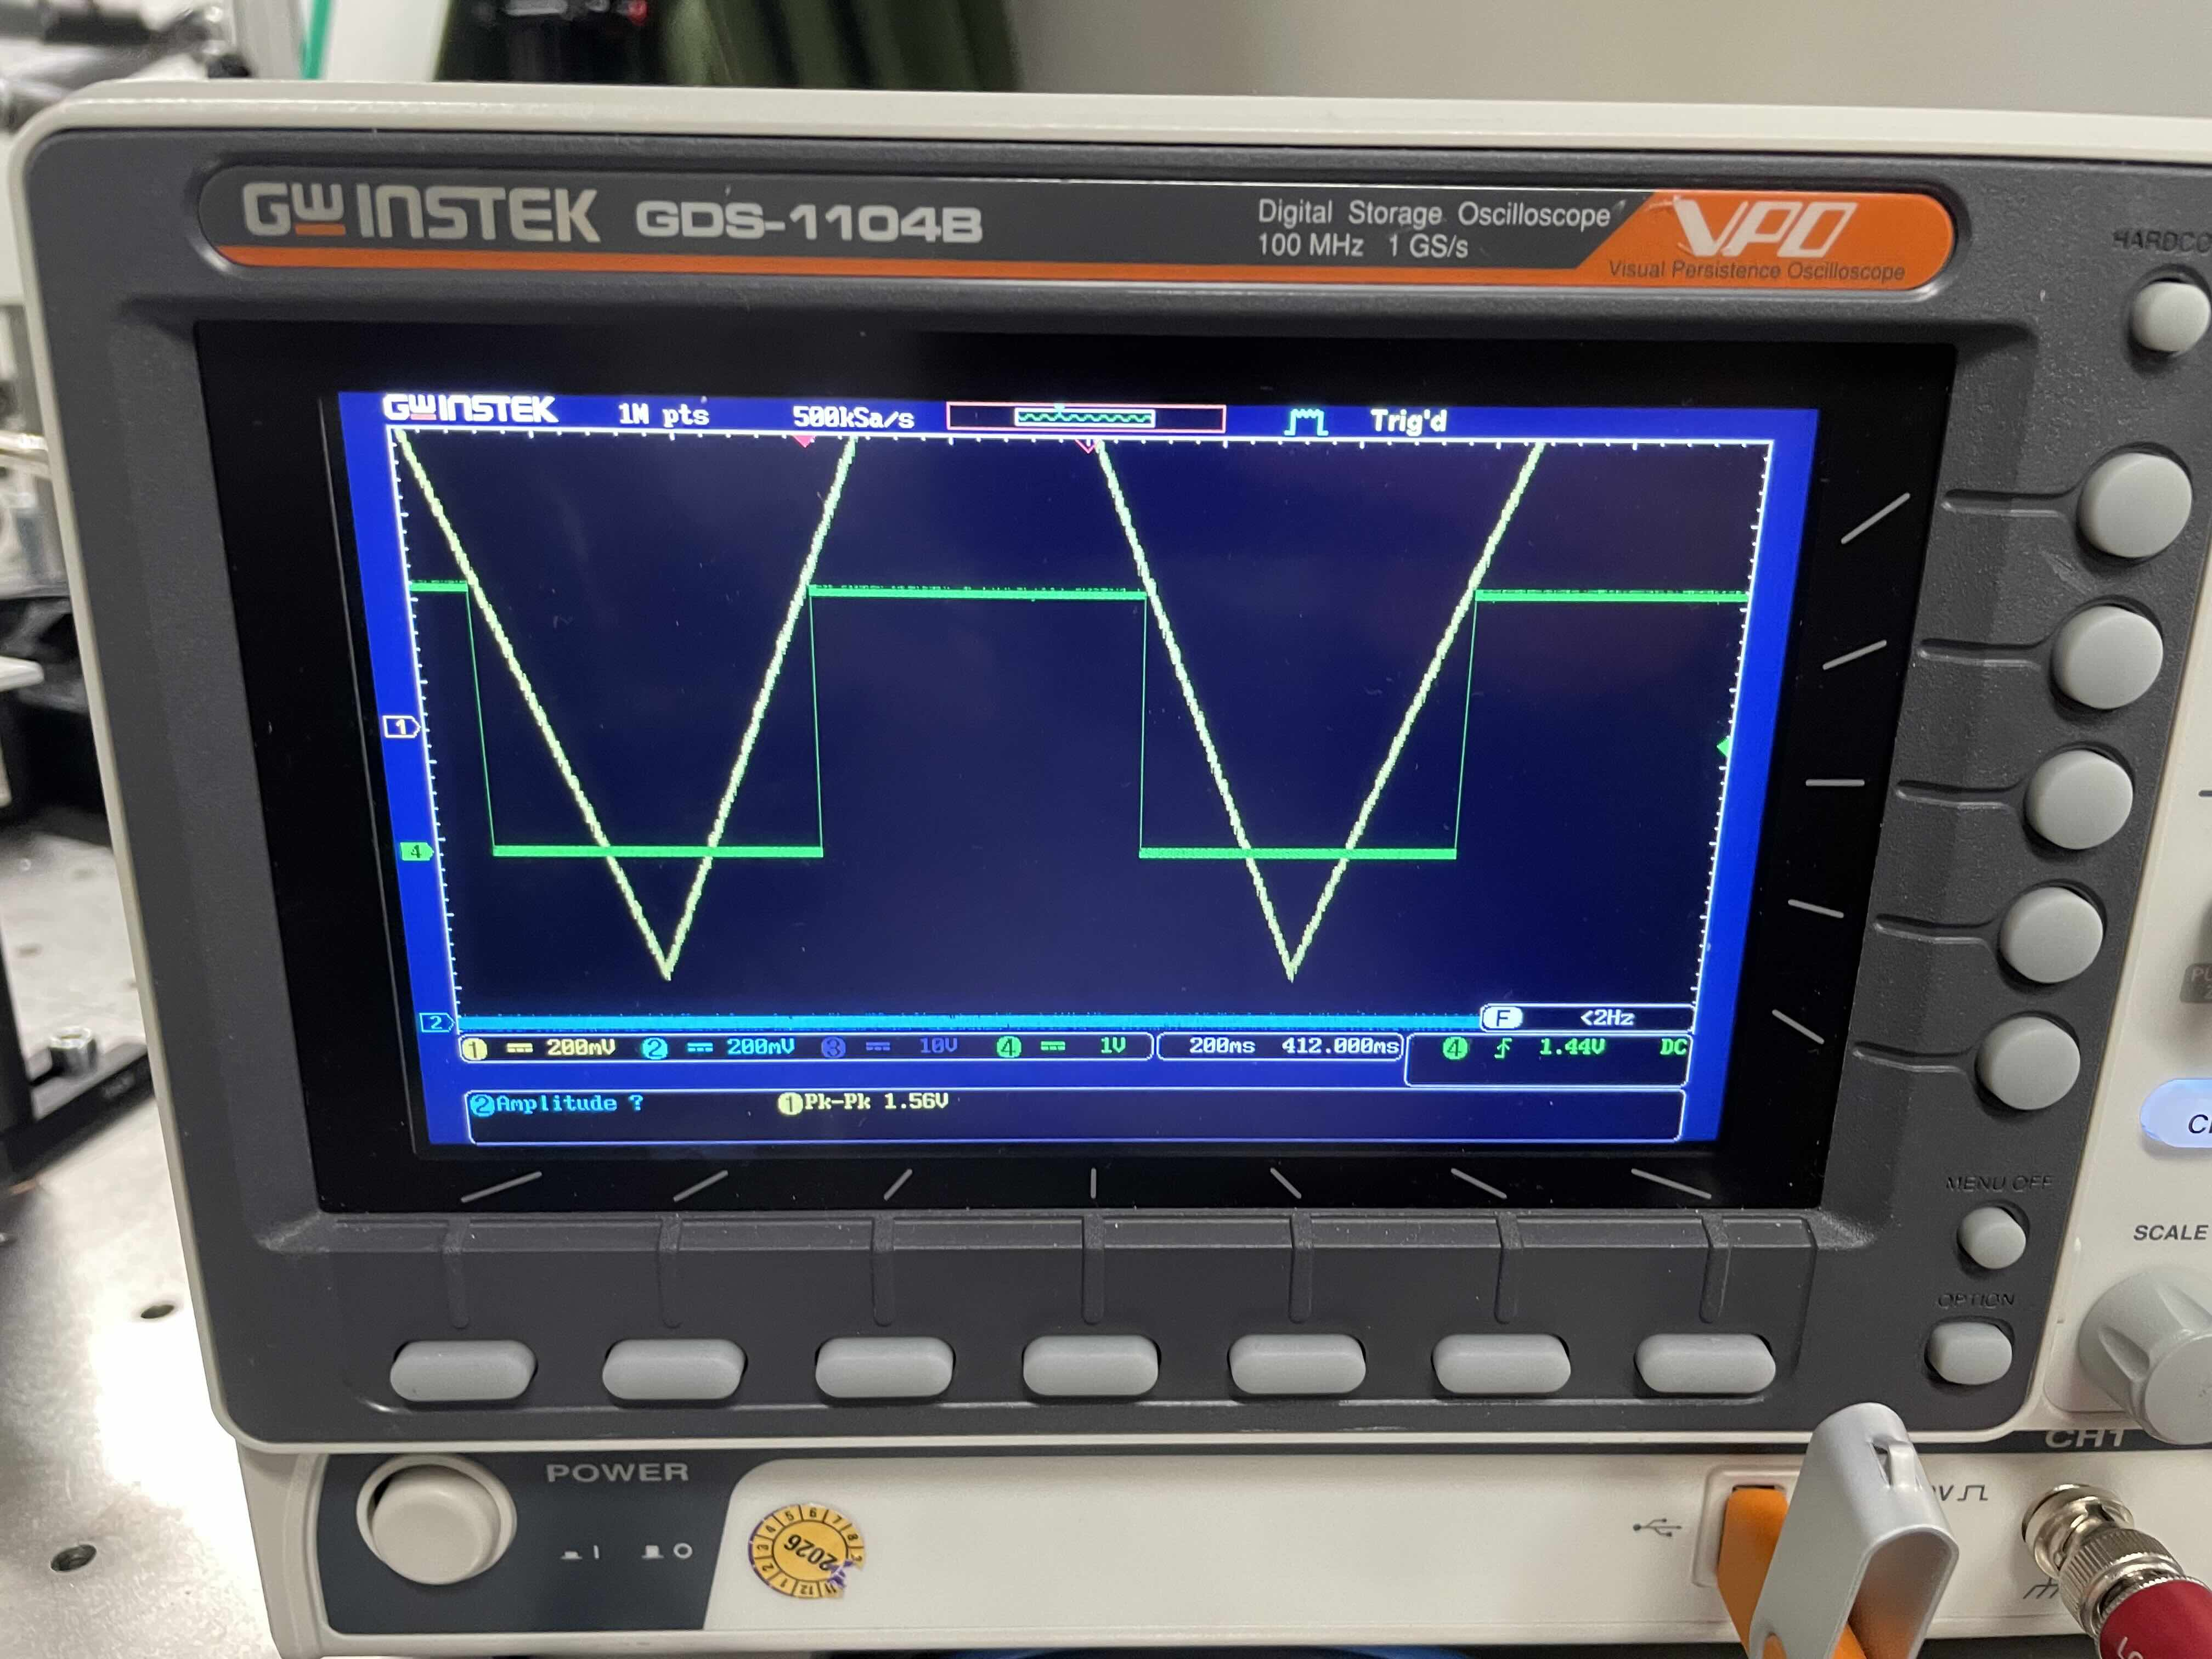
\includegraphics[width=\textwidth]{osci.jpeg}
    \caption{Sync voltage vs piezo driver voltage.}
    \label{fig:osci}
\end{figure}




\end{document}